\documentclass[12pt, a4paper,twoside]{article}
% \usepackage{nicefrac}
% \usepackage[lmargin=3cm,rmargin=2.1cm,tmargin=2.4cm,bmargin=2.4cm]{geometry}
\begin{document}
\label{sec:workBefore}
	I had done some Literature review to proposed a proper solution for the problem. Literature review was mainly done for two parts: (1) Aligning images and (2) How to generate binary vectors.

	To deal with the non-aligned images, according to the paper \cite{align} I am using a convolutional neural network architecture for estimating parameters of a geometric transformation between two input images.The classical approach consists of the following stages: (i) local descriptors (e.g. SIFT) are extracted from both input images, (ii) the descriptors are matched across images to form a set of tentative correspondences, which are then used to (iii) robustly estimate the parameters of the geometric model using RANSAC or Hough voting \cite{34b}.

\begin{figure}[htbp]
\centering
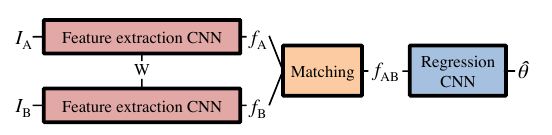
\includegraphics[scale=0.5]{images/AlignmentNetwork}
\caption{ Diagram of the architecture.
}\label{fig:figure3}
\end{figure} 

	The architecture used in this project mimics this process by: (i) passing input images $I_{A}$ and $I_{B}$ through a siamese architecture consisting of convolutional layers, thus extracting feature maps $f_{A}$ and $f_{B}$ which are analogous to dense local descriptors, (ii) matching the feature maps (“descriptors”) across images into a tentative correspondence map $f_{AB}$ , followed by a (iii) regression network which directly outputs the parameters of the geometric model, θ̂, in a robust manner. The inputs to the network are the two images, and the outputs are the parameters of the chosen geometric model, e.g. a 6-D vector for an affine transformation.

\begin{itemize}
  \item Feature Extraction

	The first stage of the pipeline is feature extraction, for which a standard CNN architecture is used. A CNN without fully connected layers takes an input image and produces a feature map f $\in$ $R^{ h\times w\times d}$ , which can be interpreted as a $h \times w$ dense spatial grid of d-dimensional local descriptors. Thus, for feature extraction we use the VGG-16 network \cite{48b}, cropped at the pool4 layer (before the ReLU unit), followed by per-feature L2-normalization.
\end{itemize}

\begin{itemize}
  \item Matching Network

\begin{figure}[htbp]
\centering
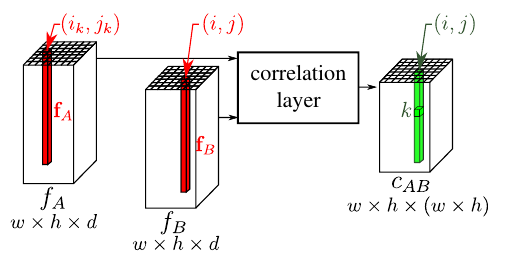
\includegraphics[scale=0.5]{images/Coreraltion}
\caption{ Correlation map computation with CNN features.
}\label{fig:figure4}
\end{figure} 

	Firstly, all pairs of similarities between descriptors are computed in the correlation layer. Secondly, similarity scores are processed and normalized such that ambiguous matches are strongly down-weighted. In more detail, given L2-normalized dense feature maps $f_{A}$ , $f_{B}$$ \in$ $R^{h\times w \times d}$ , the correlation map $c_{AB} \in$$R^{h\times w\times (h\times w)}$ outputted by the correlation layer contains at each position the scalar product of a pair of individual descriptors $f_{A} \in f_{A}$ and $f_{B} \in f_{B}$ , as detailed in Eq. (1).
	\begin{equation}
		c_{AB} (i,j,k)= f_{B} (i, j)^{T} f_{A}(i_{k}, j_{k})
        \label{eq1}
    \end{equation}
	(1) where (i, j) and $(i_{k} , j_{k} )$ indicate the individual feature positions in the h×w dense feature maps, and $k = h(j_{k} - 1)+i_{k}$ is an auxiliary indexing variable for $(i_{k} , j_{k} )$. A diagram of the correlation layer is presented in Fig~\ref{fig:figure4}. Note that at a particular position (i, j), the correlation map $c_{AB}$ contains the similarities between $f_{B}$ at that position and all the features of $f_{A}$. The normalization is performed by ReLU, to zero out negative correlations,followed by L2-normalization.

\end{itemize}

\begin{itemize}
  \item Regression Network

\begin{figure}[htbp]
\centering
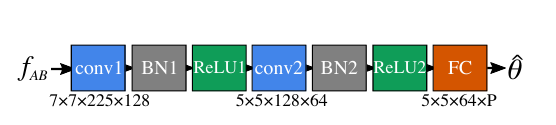
\includegraphics[scale=0.5]{images/regression}
\caption{ Architecture of the regression network.
}\label{fig:figure5}
\end{figure} 
	The normalized correlation map is passed through a regression network which directly estimates parameters of the geometric transformation relating the two input images. Now the two blocks of convolutional layers have been stacked together, followed by batch normalization and the ReLU non-linearity, and add a final fully connected layer which regresses to the parameters of the transformation, as shown in Fig~\ref{fig:figure5}. The intuition behind this architecture is that the estimation is performed in a bottom-up manner, where early convolutional layers vote for candidate transformations, and these are then processed by the later layers to aggregate the votes. The first convolutional layers can also enforce local neighborhood consensus by learning filters which only fire if nearby descriptors in image A are matched to nearby descriptors in image B.

\end{itemize}

	Now after successfull alignment of images, we come back to our deep hashing part. The proposed network after hashing is as shown in Fig~\ref{fig:figure6}
 
\begin{figure}[htbp]
\centering
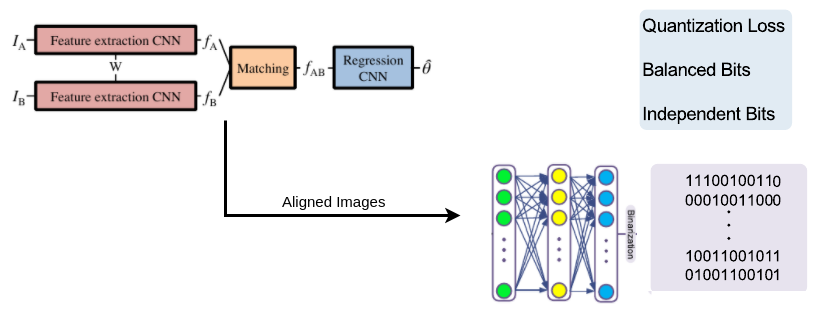
\includegraphics[scale=0.5]{images/MainNetwork}
\caption{ Architecture of the proposed network.
}\label{fig:figure6}
\end{figure} 

	For deep hashing I am refereing the following paper\cite{DeepHashing}. They have used two different approaches for hashing 1) Deep Hashing and 2) Supervised Deep Hashing. 

\begin{itemize}
  \item Deep Hashing

	The procedure of Deep Hashing used by them can be stated as:

	Let  $X = [x_{1}, x_{2} , · · · , x_{N} ] \in R^{d\times N}$ be the training set which contains N samples, where $x_{n} \in R^{d} (1 \leq n \leq N)$  is the nth sample in X.Assume there be a K hashing functions to be learned, which map $x_{n}$ into a K-bit binary codes vector  $b_{n} = [b_{n1} , · · · , b_{nK} ] \in {−1, 1}^{K \times 1}$, and the kth binary bit $b_{nk}$ of $x_{n}$ is computed as follows:

	\begin{equation}
        b_{nk} = f_{k} (x_{n} ) = sgn(g_{k}(x_{n})) = sgn(w_{k}^{T}x_{n})
        \label{eq2}
    \end{equation}
  
	where $f_{k}$ is the kth hashing function, and $w_{k} \in R^{d}$ is the projection in $f_{k} , sgn(v)$ returns $1$ if $v > 0$ and $-1$ otherwise. Let $W = [w_{1} , w_{2} , · · · , w_{K} ] \in R^{d\times K}$ be the projection matrix. Hence the final output of top layer of the network is 

	\begin{equation}
        g_{DH}(x_{n}) = h^{M} = s(W^{M}h_{n}^{M-1}+c^{M})
        \label{eq3}
    \end{equation}

    where the mapping $g_{DH}:R^{d}\rightarrow R^{p^{M}}$ is parameterized by {W m , cm }m=1 M , 1 ≤ m ≤ M, $h_{M}$ is defined as the compact realvalued code learned from several nonlinear transformations of the original feature with specific constraints. 
\end{itemize}

\end{document} 
